% Created by tikzDevice version 0.11 on 2018-10-06 09:33:43
% !TEX encoding = UTF-8 Unicode
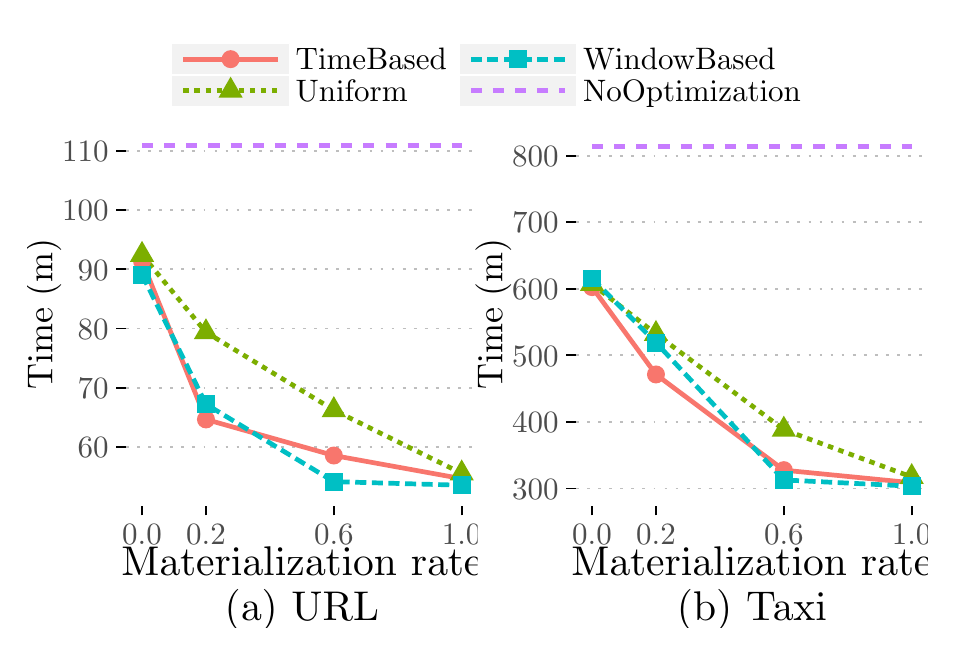
\begin{tikzpicture}[x=1pt,y=1pt]
\definecolor{fillColor}{RGB}{255,255,255}
\path[use as bounding box,fill=fillColor,fill opacity=0.00] (0,0) rectangle (325.21,216.81);
\begin{scope}
\path[clip] (  0.00,  0.00) rectangle (325.21,216.81);
\definecolor{fillColor}{RGB}{255,255,255}

\path[fill=fillColor] ( 41.96,182.67) rectangle (283.25,216.81);
\end{scope}
\begin{scope}
\path[clip] (  0.00,  0.00) rectangle (325.21,216.81);
\definecolor{drawColor}{RGB}{255,255,255}
\definecolor{fillColor}{gray}{0.95}

\path[draw=drawColor,line width= 0.6pt,line join=round,line cap=round,fill=fillColor] ( 51.99,199.74) rectangle ( 94.67,211.12);
\end{scope}
\begin{scope}
\path[clip] (  0.00,  0.00) rectangle (325.21,216.81);
\definecolor{drawColor}{RGB}{248,118,109}

\path[draw=drawColor,line width= 1.7pt,line join=round] ( 56.26,205.43) -- ( 90.40,205.43);
\end{scope}
\begin{scope}
\path[clip] (  0.00,  0.00) rectangle (325.21,216.81);
\definecolor{fillColor}{RGB}{248,118,109}

\path[fill=fillColor] ( 73.33,205.43) circle (  3.25);
\end{scope}
\begin{scope}
\path[clip] (  0.00,  0.00) rectangle (325.21,216.81);
\definecolor{drawColor}{RGB}{255,255,255}
\definecolor{fillColor}{gray}{0.95}

\path[draw=drawColor,line width= 0.6pt,line join=round,line cap=round,fill=fillColor] ( 51.99,188.36) rectangle ( 94.67,199.74);
\end{scope}
\begin{scope}
\path[clip] (  0.00,  0.00) rectangle (325.21,216.81);
\definecolor{drawColor}{RGB}{124,174,0}

\path[draw=drawColor,line width= 1.7pt,dash pattern=on 2pt off 2pt ,line join=round] ( 56.26,194.05) -- ( 90.40,194.05);
\end{scope}
\begin{scope}
\path[clip] (  0.00,  0.00) rectangle (325.21,216.81);
\definecolor{fillColor}{RGB}{124,174,0}

\path[fill=fillColor] ( 73.33,199.10) --
	( 77.70,191.52) --
	( 68.96,191.52) --
	cycle;
\end{scope}
\begin{scope}
\path[clip] (  0.00,  0.00) rectangle (325.21,216.81);
\definecolor{drawColor}{RGB}{255,255,255}
\definecolor{fillColor}{gray}{0.95}

\path[draw=drawColor,line width= 0.6pt,line join=round,line cap=round,fill=fillColor] (155.86,199.74) rectangle (198.54,211.12);
\end{scope}
\begin{scope}
\path[clip] (  0.00,  0.00) rectangle (325.21,216.81);
\definecolor{drawColor}{RGB}{0,191,196}

\path[draw=drawColor,line width= 1.7pt,dash pattern=on 4pt off 2pt ,line join=round] (160.13,205.43) -- (194.27,205.43);
\end{scope}
\begin{scope}
\path[clip] (  0.00,  0.00) rectangle (325.21,216.81);
\definecolor{fillColor}{RGB}{0,191,196}

\path[fill=fillColor] (173.96,202.18) --
	(180.45,202.18) --
	(180.45,208.68) --
	(173.96,208.68) --
	cycle;
\end{scope}
\begin{scope}
\path[clip] (  0.00,  0.00) rectangle (325.21,216.81);
\definecolor{drawColor}{RGB}{255,255,255}
\definecolor{fillColor}{gray}{0.95}

\path[draw=drawColor,line width= 0.6pt,line join=round,line cap=round,fill=fillColor] (155.86,188.36) rectangle (198.54,199.74);
\end{scope}
\begin{scope}
\path[clip] (  0.00,  0.00) rectangle (325.21,216.81);
\definecolor{drawColor}{RGB}{199,124,255}

\path[draw=drawColor,line width= 1.7pt,dash pattern=on 4pt off 4pt ,line join=round] (160.13,194.05) -- (194.27,194.05);
\end{scope}
\begin{scope}
\path[clip] (  0.00,  0.00) rectangle (325.21,216.81);
\definecolor{drawColor}{RGB}{0,0,0}

\node[text=drawColor,anchor=base west,inner sep=0pt, outer sep=0pt, scale=  1.12] at ( 96.84,201.57) {TimeBased};
\end{scope}
\begin{scope}
\path[clip] (  0.00,  0.00) rectangle (325.21,216.81);
\definecolor{drawColor}{RGB}{0,0,0}

\node[text=drawColor,anchor=base west,inner sep=0pt, outer sep=0pt, scale=  1.12] at ( 96.84,190.19) {Uniform};
\end{scope}
\begin{scope}
\path[clip] (  0.00,  0.00) rectangle (325.21,216.81);
\definecolor{drawColor}{RGB}{0,0,0}

\node[text=drawColor,anchor=base west,inner sep=0pt, outer sep=0pt, scale=  1.12] at (200.71,201.57) {WindowBased};
\end{scope}
\begin{scope}
\path[clip] (  0.00,  0.00) rectangle (325.21,216.81);
\definecolor{drawColor}{RGB}{0,0,0}

\node[text=drawColor,anchor=base west,inner sep=0pt, outer sep=0pt, scale=  1.12] at (200.71,190.19) {NoOptimization};
\end{scope}
\begin{scope}
\path[clip] (  0.00,  0.00) rectangle (162.61,182.67);
\definecolor{drawColor}{RGB}{255,255,255}
\definecolor{fillColor}{RGB}{255,255,255}

\path[draw=drawColor,line width= 0.6pt,line join=round,line cap=round,fill=fillColor] (  0.00,  0.00) rectangle (162.61,182.67);
\end{scope}
\begin{scope}
\path[clip] ( 35.54, 44.04) rectangle (162.61,182.67);
\definecolor{fillColor}{RGB}{255,255,255}

\path[fill=fillColor] ( 35.54, 44.04) rectangle (162.61,182.67);
\definecolor{drawColor}{RGB}{255,255,255}

\path[draw=drawColor,line width= 0.3pt,line join=round] ( 35.54, 54.62) --
	(162.61, 54.62);

\path[draw=drawColor,line width= 0.3pt,line join=round] ( 35.54, 76.01) --
	(162.61, 76.01);

\path[draw=drawColor,line width= 0.3pt,line join=round] ( 35.54, 97.40) --
	(162.61, 97.40);

\path[draw=drawColor,line width= 0.3pt,line join=round] ( 35.54,118.80) --
	(162.61,118.80);

\path[draw=drawColor,line width= 0.3pt,line join=round] ( 35.54,140.19) --
	(162.61,140.19);

\path[draw=drawColor,line width= 0.3pt,line join=round] ( 35.54,161.58) --
	(162.61,161.58);

\path[draw=drawColor,line width= 0.3pt,line join=round] ( 52.87, 44.04) --
	( 52.87,182.67);

\path[draw=drawColor,line width= 0.3pt,line join=round] ( 87.52, 44.04) --
	( 87.52,182.67);

\path[draw=drawColor,line width= 0.3pt,line join=round] (133.73, 44.04) --
	(133.73,182.67);
\definecolor{drawColor}{RGB}{190,190,190}

\path[draw=drawColor,line width= 0.6pt,dash pattern=on 1pt off 3pt ,line join=round] ( 35.54, 65.31) --
	(162.61, 65.31);

\path[draw=drawColor,line width= 0.6pt,dash pattern=on 1pt off 3pt ,line join=round] ( 35.54, 86.71) --
	(162.61, 86.71);

\path[draw=drawColor,line width= 0.6pt,dash pattern=on 1pt off 3pt ,line join=round] ( 35.54,108.10) --
	(162.61,108.10);

\path[draw=drawColor,line width= 0.6pt,dash pattern=on 1pt off 3pt ,line join=round] ( 35.54,129.49) --
	(162.61,129.49);

\path[draw=drawColor,line width= 0.6pt,dash pattern=on 1pt off 3pt ,line join=round] ( 35.54,150.88) --
	(162.61,150.88);

\path[draw=drawColor,line width= 0.6pt,dash pattern=on 1pt off 3pt ,line join=round] ( 35.54,172.28) --
	(162.61,172.28);
\definecolor{drawColor}{RGB}{255,255,255}

\path[draw=drawColor,line width= 0.6pt,line join=round] ( 41.32, 44.04) --
	( 41.32,182.67);

\path[draw=drawColor,line width= 0.6pt,line join=round] ( 64.42, 44.04) --
	( 64.42,182.67);

\path[draw=drawColor,line width= 0.6pt,line join=round] (110.63, 44.04) --
	(110.63,182.67);

\path[draw=drawColor,line width= 0.6pt,line join=round] (156.83, 44.04) --
	(156.83,182.67);
\definecolor{drawColor}{RGB}{248,118,109}

\path[draw=drawColor,line width= 1.7pt,line join=round] ( 41.32,132.48) --
	( 64.42, 75.25) --
	(110.63, 62.21) --
	(156.83, 53.84);
\definecolor{drawColor}{RGB}{124,174,0}

\path[draw=drawColor,line width= 1.7pt,dash pattern=on 2pt off 2pt ,line join=round] ( 41.32,134.74) --
	( 64.42,106.77) --
	(110.63, 78.64) --
	(156.83, 55.76);
\definecolor{drawColor}{RGB}{0,191,196}

\path[draw=drawColor,line width= 1.7pt,dash pattern=on 4pt off 2pt ,line join=round] ( 41.32,127.61) --
	( 64.42, 80.76) --
	(110.63, 52.76) --
	(156.83, 51.47);
\definecolor{drawColor}{RGB}{199,124,255}

\path[draw=drawColor,line width= 1.7pt,dash pattern=on 4pt off 4pt ,line join=round] ( 41.32,174.23) --
	( 64.42,174.23) --
	(110.63,174.23) --
	(156.83,174.23);
\definecolor{fillColor}{RGB}{248,118,109}

\path[fill=fillColor] ( 41.32,132.48) circle (  3.25);

\path[fill=fillColor] ( 64.42, 75.25) circle (  3.25);

\path[fill=fillColor] (110.63, 62.21) circle (  3.25);

\path[fill=fillColor] (156.83, 53.84) circle (  3.25);
\definecolor{fillColor}{RGB}{124,174,0}

\path[fill=fillColor] ( 41.32,139.79) --
	( 45.69,132.21) --
	( 36.94,132.21) --
	cycle;

\path[fill=fillColor] ( 64.42,111.82) --
	( 68.79,104.25) --
	( 60.05,104.25) --
	cycle;

\path[fill=fillColor] (110.63, 83.69) --
	(115.00, 76.11) --
	(106.25, 76.11) --
	cycle;

\path[fill=fillColor] (156.83, 60.81) --
	(161.21, 53.23) --
	(152.46, 53.23) --
	cycle;
\definecolor{fillColor}{RGB}{0,191,196}

\path[fill=fillColor] ( 38.07,124.36) --
	( 44.57,124.36) --
	( 44.57,130.86) --
	( 38.07,130.86) --
	cycle;

\path[fill=fillColor] ( 61.17, 77.52) --
	( 67.67, 77.52) --
	( 67.67, 84.01) --
	( 61.17, 84.01) --
	cycle;

\path[fill=fillColor] (107.38, 49.51) --
	(113.87, 49.51) --
	(113.87, 56.01) --
	(107.38, 56.01) --
	cycle;

\path[fill=fillColor] (153.58, 48.22) --
	(160.08, 48.22) --
	(160.08, 54.72) --
	(153.58, 54.72) --
	cycle;
\end{scope}
\begin{scope}
\path[clip] (  0.00,  0.00) rectangle (325.21,216.81);
\definecolor{drawColor}{gray}{0.30}

\node[text=drawColor,anchor=base east,inner sep=0pt, outer sep=0pt, scale=  1.12] at ( 29.24, 61.46) {60};

\node[text=drawColor,anchor=base east,inner sep=0pt, outer sep=0pt, scale=  1.12] at ( 29.24, 82.85) {70};

\node[text=drawColor,anchor=base east,inner sep=0pt, outer sep=0pt, scale=  1.12] at ( 29.24,104.24) {80};

\node[text=drawColor,anchor=base east,inner sep=0pt, outer sep=0pt, scale=  1.12] at ( 29.24,125.63) {90};

\node[text=drawColor,anchor=base east,inner sep=0pt, outer sep=0pt, scale=  1.12] at ( 29.24,147.03) {100};

\node[text=drawColor,anchor=base east,inner sep=0pt, outer sep=0pt, scale=  1.12] at ( 29.24,168.42) {110};
\end{scope}
\begin{scope}
\path[clip] (  0.00,  0.00) rectangle (325.21,216.81);
\definecolor{drawColor}{RGB}{0,0,0}

\path[draw=drawColor,line width= 0.6pt,line join=round] ( 32.04, 65.31) --
	( 35.54, 65.31);

\path[draw=drawColor,line width= 0.6pt,line join=round] ( 32.04, 86.71) --
	( 35.54, 86.71);

\path[draw=drawColor,line width= 0.6pt,line join=round] ( 32.04,108.10) --
	( 35.54,108.10);

\path[draw=drawColor,line width= 0.6pt,line join=round] ( 32.04,129.49) --
	( 35.54,129.49);

\path[draw=drawColor,line width= 0.6pt,line join=round] ( 32.04,150.88) --
	( 35.54,150.88);

\path[draw=drawColor,line width= 0.6pt,line join=round] ( 32.04,172.28) --
	( 35.54,172.28);
\end{scope}
\begin{scope}
\path[clip] (  0.00,  0.00) rectangle (325.21,216.81);
\definecolor{drawColor}{RGB}{0,0,0}

\path[draw=drawColor,line width= 0.6pt,line join=round] ( 41.32, 40.54) --
	( 41.32, 44.04);

\path[draw=drawColor,line width= 0.6pt,line join=round] ( 64.42, 40.54) --
	( 64.42, 44.04);

\path[draw=drawColor,line width= 0.6pt,line join=round] (110.63, 40.54) --
	(110.63, 44.04);

\path[draw=drawColor,line width= 0.6pt,line join=round] (156.83, 40.54) --
	(156.83, 44.04);
\end{scope}
\begin{scope}
\path[clip] (  0.00,  0.00) rectangle (325.21,216.81);
\definecolor{drawColor}{gray}{0.30}

\node[text=drawColor,anchor=base,inner sep=0pt, outer sep=0pt, scale=  1.12] at ( 41.32, 30.02) {0.0};

\node[text=drawColor,anchor=base,inner sep=0pt, outer sep=0pt, scale=  1.12] at ( 64.42, 30.02) {0.2};

\node[text=drawColor,anchor=base,inner sep=0pt, outer sep=0pt, scale=  1.12] at (110.63, 30.02) {0.6};

\node[text=drawColor,anchor=base,inner sep=0pt, outer sep=0pt, scale=  1.12] at (156.83, 30.02) {1.0};
\end{scope}
\begin{scope}
\path[clip] (  0.00,  0.00) rectangle (325.21,216.81);
\definecolor{drawColor}{RGB}{0,0,0}

\node[text=drawColor,anchor=base,inner sep=0pt, outer sep=0pt, scale=  1.50] at ( 99.08, 18.69) {Materialization rate};

\node[text=drawColor,anchor=base,inner sep=0pt, outer sep=0pt, scale=  1.50] at ( 99.08,  2.49) { (a) URL};
\end{scope}
\begin{scope}
\path[clip] (  0.00,  0.00) rectangle (325.21,216.81);
\definecolor{drawColor}{RGB}{0,0,0}

\node[text=drawColor,rotate= 90.00,anchor=base,inner sep=0pt, outer sep=0pt, scale=  1.30] at (  8.95,113.35) {Time (m)};
\end{scope}
\begin{scope}
\path[clip] (162.61,  0.00) rectangle (325.21,182.67);
\definecolor{drawColor}{RGB}{255,255,255}
\definecolor{fillColor}{RGB}{255,255,255}

\path[draw=drawColor,line width= 0.6pt,line join=round,line cap=round,fill=fillColor] (162.61,  0.00) rectangle (325.21,182.67);
\end{scope}
\begin{scope}
\path[clip] (198.15, 44.04) rectangle (325.21,182.67);
\definecolor{fillColor}{RGB}{255,255,255}

\path[fill=fillColor] (198.15, 44.04) rectangle (325.21,182.67);
\definecolor{drawColor}{RGB}{255,255,255}

\path[draw=drawColor,line width= 0.3pt,line join=round] (198.15, 62.36) --
	(325.21, 62.36);

\path[draw=drawColor,line width= 0.3pt,line join=round] (198.15, 86.39) --
	(325.21, 86.39);

\path[draw=drawColor,line width= 0.3pt,line join=round] (198.15,110.43) --
	(325.21,110.43);

\path[draw=drawColor,line width= 0.3pt,line join=round] (198.15,134.46) --
	(325.21,134.46);

\path[draw=drawColor,line width= 0.3pt,line join=round] (198.15,158.50) --
	(325.21,158.50);

\path[draw=drawColor,line width= 0.3pt,line join=round] (198.15,182.53) --
	(325.21,182.53);

\path[draw=drawColor,line width= 0.3pt,line join=round] (215.48, 44.04) --
	(215.48,182.67);

\path[draw=drawColor,line width= 0.3pt,line join=round] (250.13, 44.04) --
	(250.13,182.67);

\path[draw=drawColor,line width= 0.3pt,line join=round] (296.34, 44.04) --
	(296.34,182.67);
\definecolor{drawColor}{RGB}{190,190,190}

\path[draw=drawColor,line width= 0.6pt,dash pattern=on 1pt off 3pt ,line join=round] (198.15, 50.34) --
	(325.21, 50.34);

\path[draw=drawColor,line width= 0.6pt,dash pattern=on 1pt off 3pt ,line join=round] (198.15, 74.37) --
	(325.21, 74.37);

\path[draw=drawColor,line width= 0.6pt,dash pattern=on 1pt off 3pt ,line join=round] (198.15, 98.41) --
	(325.21, 98.41);

\path[draw=drawColor,line width= 0.6pt,dash pattern=on 1pt off 3pt ,line join=round] (198.15,122.44) --
	(325.21,122.44);

\path[draw=drawColor,line width= 0.6pt,dash pattern=on 1pt off 3pt ,line join=round] (198.15,146.48) --
	(325.21,146.48);

\path[draw=drawColor,line width= 0.6pt,dash pattern=on 1pt off 3pt ,line join=round] (198.15,170.51) --
	(325.21,170.51);
\definecolor{drawColor}{RGB}{255,255,255}

\path[draw=drawColor,line width= 0.6pt,line join=round] (203.93, 44.04) --
	(203.93,182.67);

\path[draw=drawColor,line width= 0.6pt,line join=round] (227.03, 44.04) --
	(227.03,182.67);

\path[draw=drawColor,line width= 0.6pt,line join=round] (273.23, 44.04) --
	(273.23,182.67);

\path[draw=drawColor,line width= 0.6pt,line join=round] (319.44, 44.04) --
	(319.44,182.67);
\definecolor{drawColor}{RGB}{248,118,109}

\path[draw=drawColor,line width= 1.7pt,line join=round] (203.93,123.06) --
	(227.03, 91.50) --
	(273.23, 56.92) --
	(319.44, 52.37);
\definecolor{drawColor}{RGB}{124,174,0}

\path[draw=drawColor,line width= 1.7pt,dash pattern=on 2pt off 2pt ,line join=round] (203.93,124.18) --
	(227.03,106.15) --
	(273.23, 71.56) --
	(319.44, 54.46);
\definecolor{drawColor}{RGB}{0,191,196}

\path[draw=drawColor,line width= 1.7pt,dash pattern=on 4pt off 2pt ,line join=round] (203.93,126.16) --
	(227.03,103.02) --
	(273.23, 53.38) --
	(319.44, 51.12);
\definecolor{drawColor}{RGB}{199,124,255}

\path[draw=drawColor,line width= 1.7pt,dash pattern=on 4pt off 4pt ,line join=round] (203.93,173.96) --
	(227.03,173.96) --
	(273.23,173.96) --
	(319.44,173.96);
\definecolor{fillColor}{RGB}{248,118,109}

\path[fill=fillColor] (203.93,123.06) circle (  3.25);

\path[fill=fillColor] (227.03, 91.50) circle (  3.25);

\path[fill=fillColor] (273.23, 56.92) circle (  3.25);

\path[fill=fillColor] (319.44, 52.37) circle (  3.25);
\definecolor{fillColor}{RGB}{124,174,0}

\path[fill=fillColor] (203.93,129.23) --
	(208.30,121.66) --
	(199.55,121.66) --
	cycle;

\path[fill=fillColor] (227.03,111.20) --
	(231.40,103.63) --
	(222.66,103.63) --
	cycle;

\path[fill=fillColor] (273.23, 76.61) --
	(277.61, 69.04) --
	(268.86, 69.04) --
	cycle;

\path[fill=fillColor] (319.44, 59.51) --
	(323.81, 51.94) --
	(315.07, 51.94) --
	cycle;
\definecolor{fillColor}{RGB}{0,191,196}

\path[fill=fillColor] (200.68,122.92) --
	(207.17,122.92) --
	(207.17,129.41) --
	(200.68,129.41) --
	cycle;

\path[fill=fillColor] (223.78, 99.77) --
	(230.28, 99.77) --
	(230.28,106.27) --
	(223.78,106.27) --
	cycle;

\path[fill=fillColor] (269.99, 50.14) --
	(276.48, 50.14) --
	(276.48, 56.63) --
	(269.99, 56.63) --
	cycle;

\path[fill=fillColor] (316.19, 47.88) --
	(322.69, 47.88) --
	(322.69, 54.37) --
	(316.19, 54.37) --
	cycle;
\end{scope}
\begin{scope}
\path[clip] (  0.00,  0.00) rectangle (325.21,216.81);
\definecolor{drawColor}{gray}{0.30}

\node[text=drawColor,anchor=base east,inner sep=0pt, outer sep=0pt, scale=  1.12] at (191.85, 46.48) {300};

\node[text=drawColor,anchor=base east,inner sep=0pt, outer sep=0pt, scale=  1.12] at (191.85, 70.52) {400};

\node[text=drawColor,anchor=base east,inner sep=0pt, outer sep=0pt, scale=  1.12] at (191.85, 94.55) {500};

\node[text=drawColor,anchor=base east,inner sep=0pt, outer sep=0pt, scale=  1.12] at (191.85,118.59) {600};

\node[text=drawColor,anchor=base east,inner sep=0pt, outer sep=0pt, scale=  1.12] at (191.85,142.62) {700};

\node[text=drawColor,anchor=base east,inner sep=0pt, outer sep=0pt, scale=  1.12] at (191.85,166.66) {800};
\end{scope}
\begin{scope}
\path[clip] (  0.00,  0.00) rectangle (325.21,216.81);
\definecolor{drawColor}{RGB}{0,0,0}

\path[draw=drawColor,line width= 0.6pt,line join=round] (194.65, 50.34) --
	(198.15, 50.34);

\path[draw=drawColor,line width= 0.6pt,line join=round] (194.65, 74.37) --
	(198.15, 74.37);

\path[draw=drawColor,line width= 0.6pt,line join=round] (194.65, 98.41) --
	(198.15, 98.41);

\path[draw=drawColor,line width= 0.6pt,line join=round] (194.65,122.44) --
	(198.15,122.44);

\path[draw=drawColor,line width= 0.6pt,line join=round] (194.65,146.48) --
	(198.15,146.48);

\path[draw=drawColor,line width= 0.6pt,line join=round] (194.65,170.51) --
	(198.15,170.51);
\end{scope}
\begin{scope}
\path[clip] (  0.00,  0.00) rectangle (325.21,216.81);
\definecolor{drawColor}{RGB}{0,0,0}

\path[draw=drawColor,line width= 0.6pt,line join=round] (203.93, 40.54) --
	(203.93, 44.04);

\path[draw=drawColor,line width= 0.6pt,line join=round] (227.03, 40.54) --
	(227.03, 44.04);

\path[draw=drawColor,line width= 0.6pt,line join=round] (273.23, 40.54) --
	(273.23, 44.04);

\path[draw=drawColor,line width= 0.6pt,line join=round] (319.44, 40.54) --
	(319.44, 44.04);
\end{scope}
\begin{scope}
\path[clip] (  0.00,  0.00) rectangle (325.21,216.81);
\definecolor{drawColor}{gray}{0.30}

\node[text=drawColor,anchor=base,inner sep=0pt, outer sep=0pt, scale=  1.12] at (203.93, 30.02) {0.0};

\node[text=drawColor,anchor=base,inner sep=0pt, outer sep=0pt, scale=  1.12] at (227.03, 30.02) {0.2};

\node[text=drawColor,anchor=base,inner sep=0pt, outer sep=0pt, scale=  1.12] at (273.23, 30.02) {0.6};

\node[text=drawColor,anchor=base,inner sep=0pt, outer sep=0pt, scale=  1.12] at (319.44, 30.02) {1.0};
\end{scope}
\begin{scope}
\path[clip] (  0.00,  0.00) rectangle (325.21,216.81);
\definecolor{drawColor}{RGB}{0,0,0}

\node[text=drawColor,anchor=base,inner sep=0pt, outer sep=0pt, scale=  1.50] at (261.68, 18.69) {Materialization rate};

\node[text=drawColor,anchor=base,inner sep=0pt, outer sep=0pt, scale=  1.50] at (261.68,  2.49) { (b) Taxi};
\end{scope}
\begin{scope}
\path[clip] (  0.00,  0.00) rectangle (325.21,216.81);
\definecolor{drawColor}{RGB}{0,0,0}

\node[text=drawColor,rotate= 90.00,anchor=base,inner sep=0pt, outer sep=0pt, scale=  1.30] at (171.56,113.35) {Time (m)};
\end{scope}
\end{tikzpicture}
